\documentclass{homework}
% \usepackage{lua-visual-debug}
\usepackage{graphicx}
\usepackage{amsmath, amssymb, amsfonts}
\usepackage[a4paper, total={6in, 8.8in}]{geometry}

\title{Practice \#3}
\subject{CS341 Introduction to Computer Networks}
\studentid{20170058}
\name{Keonwoo Kim}
\date{\today}

\begin{document}
\maketitle

\vspace*{-4em}

\section*{Task 1}

\parindent=0pt

\solution[1.1]{
    Scenario 1: When app (a) is running (skeleton code).

    1.1.1. Plot the \textit{cwnd} (congestion window) of app (a) on a graph.

    \begin{figure*}[!h]
        \centering
        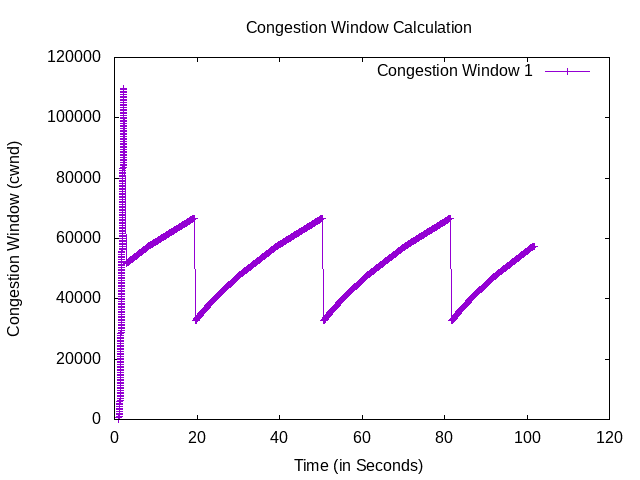
\includegraphics[width=.65\textwidth]{gnuplots/prac3.1.1.cwnd.png}
    \end{figure*}

    1.1.2. Plot the TCP throughput of app (a) in each 0.1 second. (unit x:sec, y:Mbps).

    \begin{figure*}[!h]
        \centering
        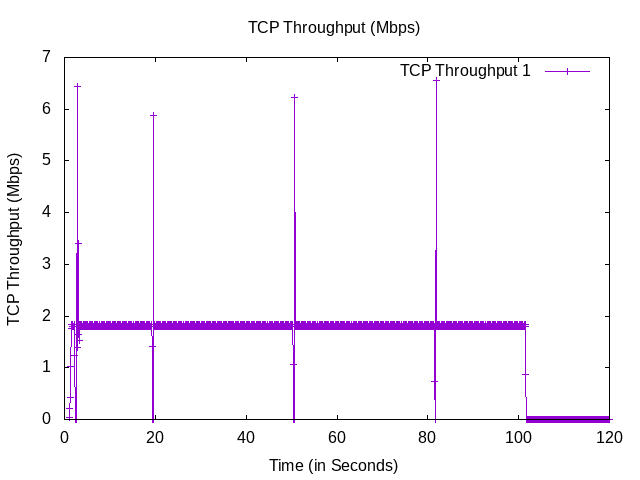
\includegraphics[width=.65\textwidth]{gnuplots/prac3.1.1.rx.png}
    \end{figure*}
}

\solution[1.2]{
    Scenario 2: When app (a, b) are running.

    1.2.1. Plot \textit{cwnd} of app (a, b) respectively on a graph. 

    \begin{figure*}[!h]
        \centering
        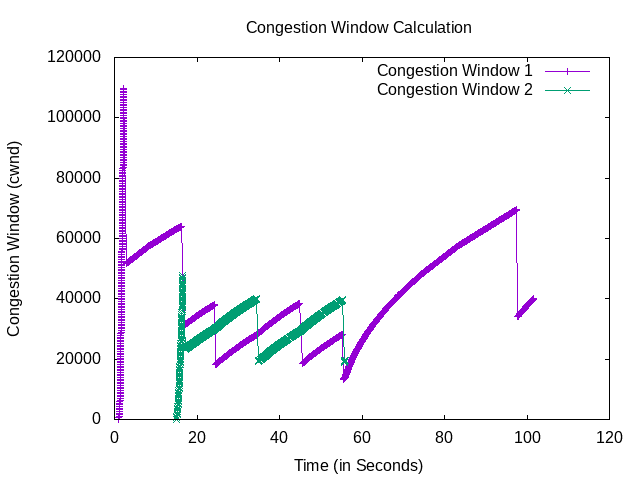
\includegraphics[width=.65\textwidth]{gnuplots/prac3.1.2.cwnd.png}
    \end{figure*}

    1.2.2. Plot the calculated TCP throughput of each app (a, b) in each 0.1 second. (unit x:sec, y:Mbps).

    \begin{figure*}[!h]
        \centering
        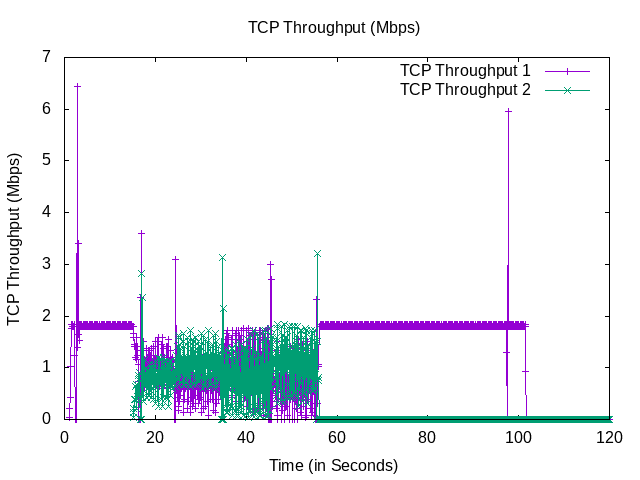
\includegraphics[width=.65\textwidth]{gnuplots/prac3.1.2.rx.png}
    \end{figure*}

    1.2.3. Describe how the graph is different from \textbf{Scenario 1 (1.1.)} and discuss the reason why.

    As there are one more application using the same link (from node 1 to node 0,) packet losses occur more frequently so the cwnd's have decreased for app (a) in comparison to one in 1.1.1. In the throughput graph, one can see that two apps are competitively sending data via the shared link. 
}

\solution[1.3]{
    Scenario 3: When app (a, b, c) are running.

    1.3.1. Plot \textit{cwnd} of app (a, b, c) respectively on a graph. 

    \begin{figure*}[!h]
        \centering
        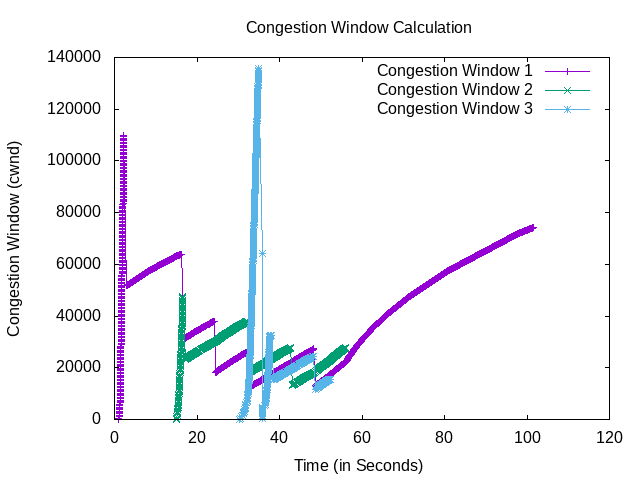
\includegraphics[width=.65\textwidth]{gnuplots/prac3.1.3.cwnd.png}
    \end{figure*}

    1.3.2. Plot the calculated TCP throughput of each app (a, b, c) in each 0.1 second. (unit x:sec, y:Mbps).

    \begin{figure*}[!h]
        \centering
        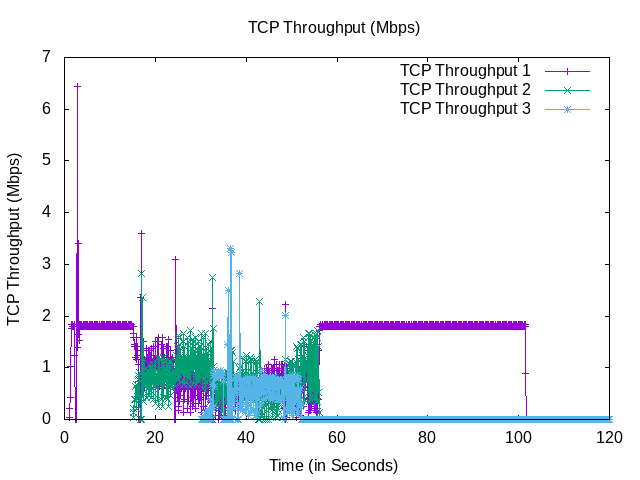
\includegraphics[width=.65\textwidth]{gnuplots/prac3.1.3.rx.png}
    \end{figure*}

    1.3.3. Describe how the graph is different from \textbf{Scenario 2 (1.2.)} and discuss the reason why.

    The reason is basically the same with one of 1.2.3., but there is one more app running from $t=30$ (s). Three apps are sending packets through the same router and the same link to the node 0, so the packet losses became more frequent and hence the level of cwnd again decreased compared to the scenario 2.
}

\solution[1.4]{
    Scenario 4: In real world scenario, there can be corrupted packets when the sink app receives the packets. On the top of Scenario 3, set the receive error rate of 1e-6 set from Node 1 to Node 0.

    1.4.1. Plot \textit{cwnd} of app (a, b, c) respectively on a graph. 

    \begin{figure*}[!h]
        \centering
        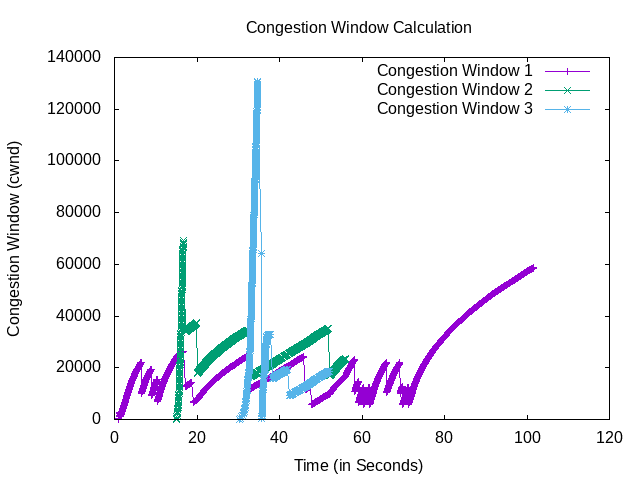
\includegraphics[width=.65\textwidth]{gnuplots/prac3.1.4.cwnd.png}
    \end{figure*}

    1.4.2. Plot the calculated TCP throughput of each app (a, b, c) in each 0.1 second. (unit x:sec, y:Mbps).

    \begin{figure*}[!h]
        \centering
        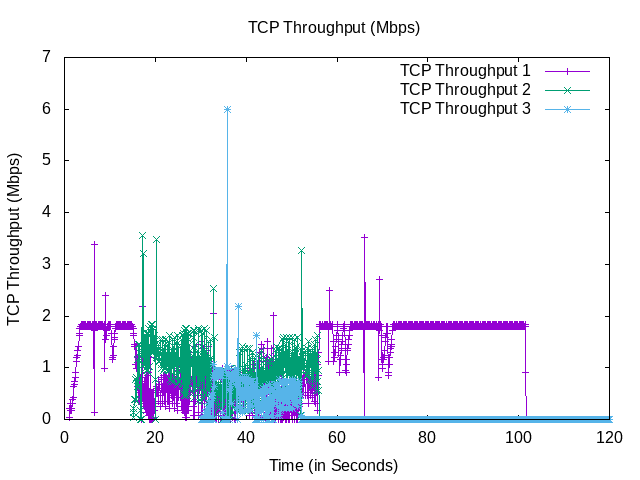
\includegraphics[width=.62\textwidth]{gnuplots/prac3.1.4.rx.png}
    \end{figure*}

    1.4.3. Describe how the graph is different from \textbf{Scenario 3 (1.3.)} and discuss the reason why.
    
    Now, packet losses occurs not only due to burst router but also by the receiver. Packet losses are again increasingly occurring, so we can see there are much more TCP recoveries presented.
}

\section*{Task 2}

\solution[2.1]{
    The default TCP congestion control algorithm in NS3 is set to \textit{TcpNewReno}, and this runs based on the \texttt{src/internet/model/tcp-congestion-ops.cc} and \texttt{src/internet/model/tcp-recovery-ops.cc}.

    2.1.1. In \texttt{tcp-congestion-ops.cc}, set the adder in \textit{CongestionAvoidance} function as Appendix 1. Plot \textit{cwnd} and TCP throughput graphs. Describe how the graph is different from \textbf{Scenario 4 (1.4.)} and discuss the reason why.

    \begin{figure*}[!h]
        \centering
        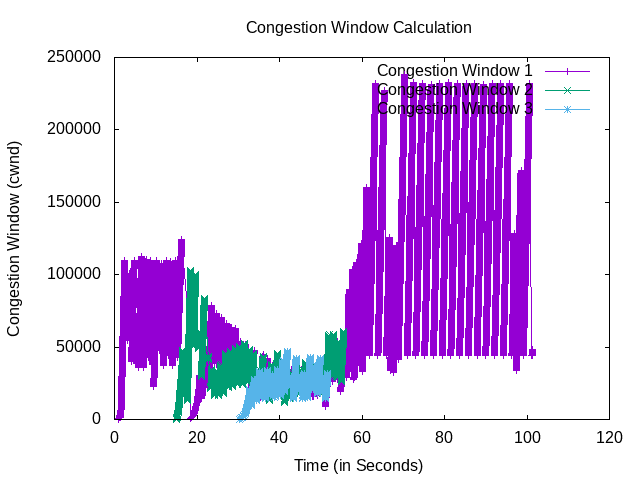
\includegraphics[width=.4\textwidth]{gnuplots/prac3.2.1.1.cwnd.png}
        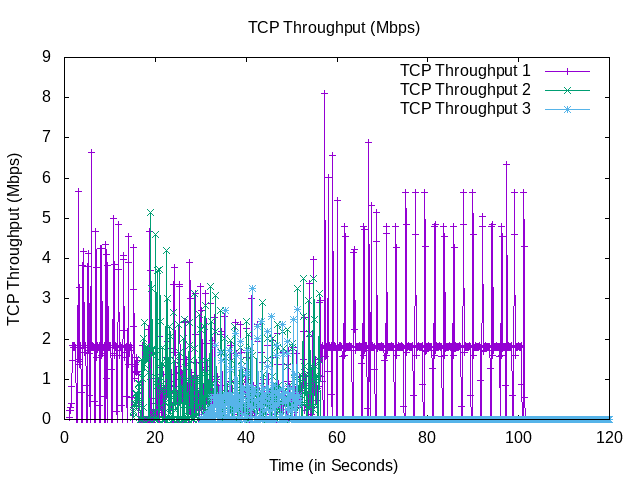
\includegraphics[width=.4\textwidth]{gnuplots/prac3.2.1.1.rx.png}
    \end{figure*}

    With the original code, we have $\Delta cwnd \text{ (or $d(cwnd)/dt$)} \propto 1/cwnd$ so that $cwnd(t) \propto \sqrt t$, this is the reason why we got a bent curve in cwnd graphs above. When we change that adder to make $\Delta cwnd \propto 1$, we have $cwnd(t) \propto t$, which means it is linear to time, with a rapid rate as the graph shows. Therefore $cwnd$ repeats to grow very rapidly and to drop due to the recovery algorithm.

    2.1.2. Roll back the changes in 2.1.1. to the original. Now in \texttt{tcp-recovery-ops.cc}, set the \textit{EnterRecover}, \textit{DoRecovery}, \textit{ExitRecovery} functions to be as Appendix 2 so that there is no recovery operation. Plot cwnd and throughput graphs. Describe how the graph is different from \textbf{Scenario 4 (1.4.)} and discuss the reason why.

    \begin{figure*}[!h]
        \centering
        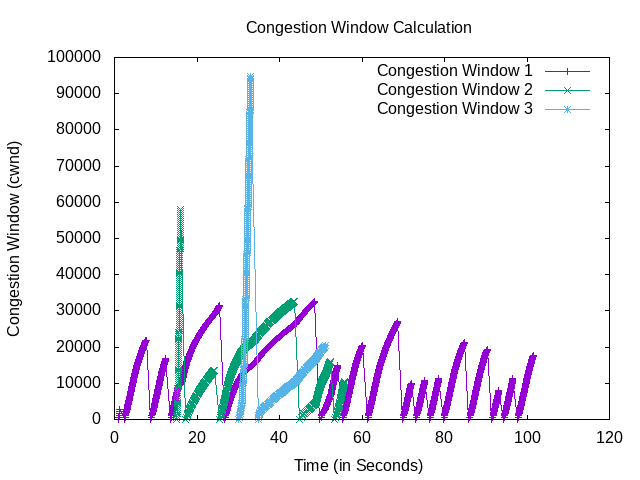
\includegraphics[width=.4\textwidth]{gnuplots/prac3.2.1.2.cwnd.png}
        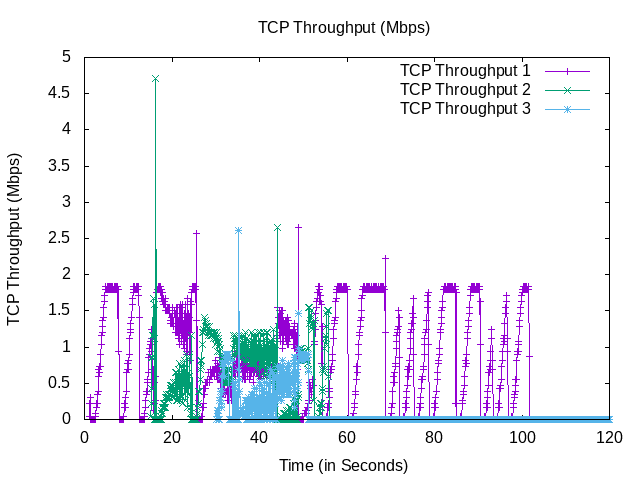
\includegraphics[width=.4\textwidth]{gnuplots/prac3.2.1.2.rx.png}
    \end{figure*}

    The modification in Appendix 2 makes $cwnd$ always be 1 after the recovery. (cWndInfl exists only for the backward compatibility.) We can see the effect of this modification easily in the cwnd graph. (Every recovery in cwnd graph starts at the very bottom, which means $cwnd=1$.)
}

\solution[2.1]{
    Roll back the previous changes in 2.1. to the original. Try \textbf{Scenario 4 (1.4)} using another TCP congestion control algorithms in NS3.

    2.2.1. Plot \textit{cwnd} and \textit{TCP} throughput graphs when the algorithm is set to \textit{Veno}.

    \begin{figure*}[!h]
        \centering
        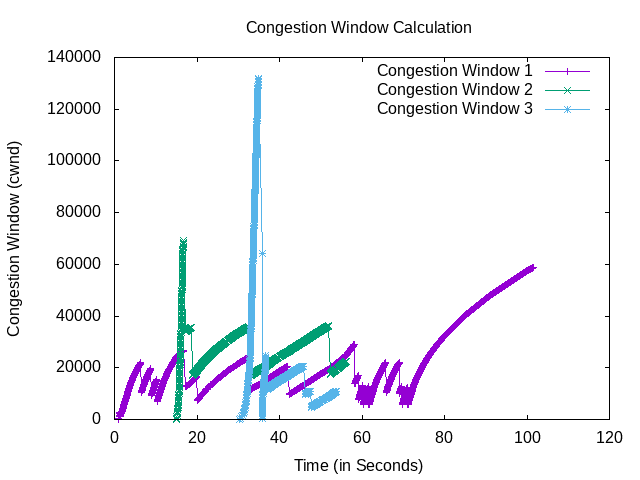
\includegraphics[width=.4\textwidth]{gnuplots/prac3.veno.cwnd.png}
        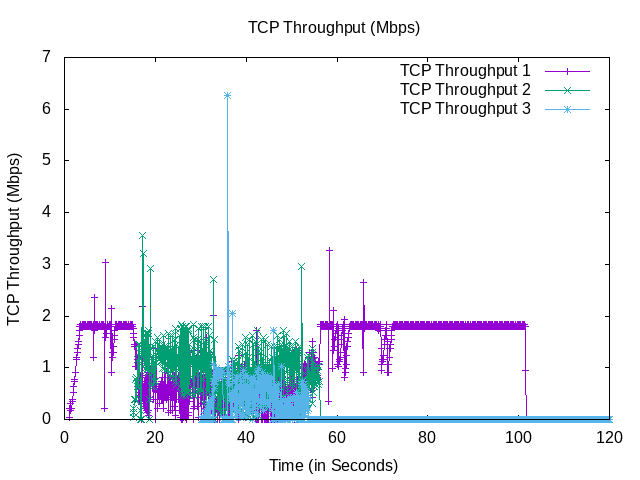
\includegraphics[width=.4\textwidth]{gnuplots/prac3.veno.rx.png}
    \end{figure*}

    2.2.2. Plot \textit{cwnd} and \textit{TCP} throughput graphs when the algorithm is set to \textit{Yeah}.

    \begin{figure*}[!h]
        \centering
        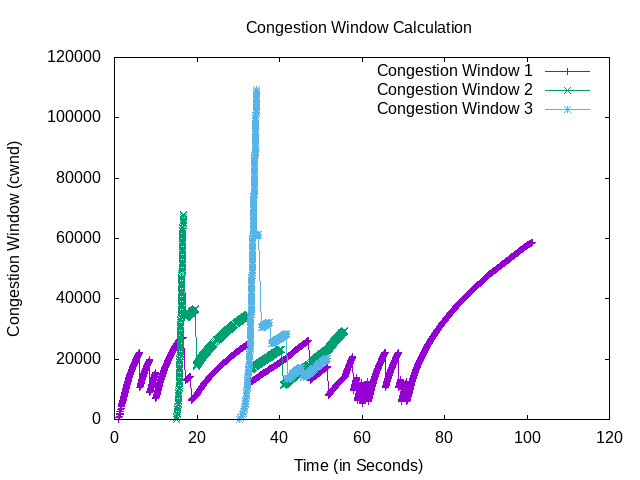
\includegraphics[width=.4\textwidth]{gnuplots/prac3.yeah.cwnd.png}
        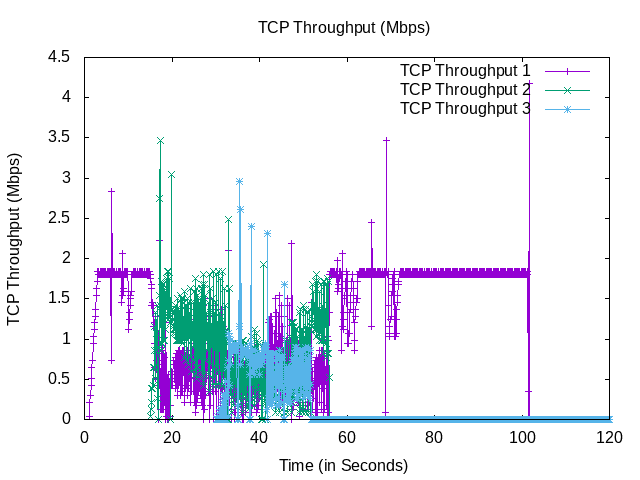
\includegraphics[width=.4\textwidth]{gnuplots/prac3.yeah.rx.png}
    \end{figure*}

    2.2.3. Record the total received bytes from the sink app of (a, b, c) respectively of the \textbf{Scenario 4} simulation on each TCP congestion algorithm: \textit{NewReno (NS3 default)}, \textit{Veno}, and \textit{Yeah}. Which algorithm do you prefer and why? Support your answer with evidence such as TCP throughput, packet loss, and congestion.

    Using flow monitor helper of ns3, we can observe the total received bytes for each app.
    \begin{table}[!h]
        \centering
        \begin{tabular}{l|rrr}
                & \textit{NewReno}  & \textit{Veno}     & \textit{Yeah}     \\ \hline
        App (a) & 17328600 & 17526020 & 17721660 \\
        App (b) & 5437312  & 5380268  & 4921760  \\
        App (c) & 1535180  & 1430460  & 1784876 
        \end{tabular}
        \caption{Table of total received bytes}
    \end{table}

    Among three, I think Yeah performs the best, as it recovers cwnd well when the network experiences a packet loss, and the total received bytes for the apps (a) and (c) are way better than other algorithms.
}



\end{document}